\documentclass{article}
%\usepackage[noenumitem]{eda} 
\usepackage{prettyplots} 
 
\usepackage{pgfplots} 
\usepackage{tikz} 
 \usepackage{eda-colors} 
 
\label{key}\pgfplotsset{compat=1.14} % tick positions
\usetikzlibrary{calc}  % Coordinate calculation
\usetikzlibrary{intersections} % Fill between
\usepgfplotslibrary{fillbetween} 
\usetikzlibrary{pgfplots.statistics} % boxplot calc
\usetikzlibrary{pgfplots.groupplots} % groups
\usepackage{numprint,fullpage}  %tkz-kiviat, spider
\usetikzlibrary{arrows} 
\usepgfplotslibrary{colorbrewer} %colormap heat
\usetikzlibrary{pgfplots.colormaps}  
\usetikzlibrary{fit}

%fonts
\usepackage[scaled]{beramono}
\usepackage[scaled]{inconsolata} 
\usepackage[T1]{fontenc}
\usepackage{fontspec}

\setmainfont{Brygada1918}[
Path=./style/BrygadaFontFiles/,
Extension = .ttf,
UprightFont=*-Regular,
BoldFont=*-Bold,
ItalicFont=*-Italic,
BoldItalicFont=*-BoldItalic
] 
%\setmonofont{JetBrainsMono}[
%Path=./style/JetbrainsFontFiles/,
%Scale=0.85,
%Extension = .ttf,
%UprightFont=*-Regular,
%BoldFont=*-Bold,
%ItalicFont=*-Italic,
%BoldItalicFont=*-BoldItalic
%] 
\setmonofont{GeistMono}[
Path=./style/Geist_Mono/static/,
Scale=0.85,
Extension = .ttf,
UprightFont=*-Regular,
BoldFont=*-Bold, 
]

%code snippets
\usepackage{listings}
\lstset{%
	basicstyle=\small\ttfamily,
	language=[LaTeX]{TeX},
	columns=fullflexible
}
\usepackage{minted}
\usemintedstyle{tango}%trac
\usepackage{tcolorbox}
\definecolor{mintedtitlebg}{RGB}{250,250,250}
\definecolor{mintedframecol}{RGB}{234,234,234}
\definecolor{mintedtitlegray}{RGB}{109,109,109}
\renewcommand{\theFancyVerbLine}{\sffamily
	\textcolor[RGB]{110,116,125}{\scriptsize
		\oldstylenums{\arabic{FancyVerbLine}}}}
\setminted{
	framesep=2mm, 
	baselinestretch=1.1,
	fontsize=\footnotesize, 
} 
\usepackage{xpatch}
\tcbset{  
	left=0pt,
	right=0pt,  
	colback=white,
	coltitle=mintedtitlegray,
	colbacktitle=mintedtitlebg,
	fonttitle=\scriptsize\ttfamily,
	boxsep=3mm,colframe=mintedframecol,
	boxrule=.2pt
} 
% code snippet boxes
\newtcolorbox{mintedicontexbox}[1][]
{ title={\raisebox{-.4mm}{\includegraphics{style/icon_tex.png}}\quad#1} }  
\newtcolorbox{mintedicontxtbox}[1][]
{ title={\raisebox{-.4mm}{\includegraphics{style/icon_data.png}}\quad#1} } 
\newtcolorbox{mintedtexbox}[1][]{ title={#1} }  
\newtcolorbox{mintedtxtbox}[1][]{ title={#1} }  

%copiability
% from http://tex.stackexchange.com/questions/57151/how-do-i-prevent-conflicts-between-accsupp-and-hyperref
\usepackage{accsupp}
\newcommand\emptyaccsupp[1]{\BeginAccSupp{ActualText={}}#1\EndAccSupp{}}
%default definition is: \def\theFancyVerbLine{\rmfamily\tiny\arabic{FancyVerbLine}}
\let\theHFancyVerbLine\theFancyVerbLine% don't apply our patch to hyperref's version
\def\theFancyVerbLine{\rmfamily\tiny\emptyaccsupp{\arabic{FancyVerbLine}}}
 
%graphics
\usepackage{graphicx}
\newlength{\bheight} 
\settoheight{\bheight}{T}
\setkeys{Gin}{height=\bheight} % includegraphics default height
\usepackage{hologo}

%title
\usepackage[nonewpage]{imakeidx}
\makeindex[title=Index,columns=1]
\title{\bfseries{PrettyPlots} \normalfont in \hologo{LaTeX}}
\author{EDA group}
%\date{May 2024}
\begin{document}
	\maketitle
	\tableofcontents
	\printindex  
	%basic plots
	\input{examples/line-experiment}
	%\begin{tikzpicture}
%\begin{axis}[
%    pretty line,  
%    ymax=10,  
%    legend entries = {Method 1, Method 2, Method 3}  
%] 
%\addlines{data/line.tsv} 
%\end{axis}
%\end{tikzpicture}   
\begin{tikzpicture}
\begin{axis}[
    pretty line,
    ymax=10,  width=\textwidth
] 
	\pgfplotsinvokeforeach{1,...,3}{
		\addplot table[x=x, y=y#1] {data/line.tsv};
		%\addlegendentry{Method #1}
	} 
\end{axis}
\end{tikzpicture}   
	\clearpage
\subsection{Box}  
\hypertarget{prettyboxplot}{}

\index{Plot Types!box}  
\index{Plot Types!box!basic}

 For box plots, you can use \texttt{pretty boxplot}.
\begin{figure}[h!]
	\begin{minipage}{0.7\textwidth}
		\begin{mintedtxtbox}[/data/box.tsv]
\begin{minted}{TeX}
%method1    ...        methodM
y1      y2      y3      y4
0.10    0.15    0.12    0.18 
... 
0.95    0.98    0.93    0.97
\end{minted}
		\end{mintedtxtbox}
\end{minipage}
\end{figure}
\begin{figure}[h!]
\begin{minipage}{0.65\textwidth} 
\begin{mintedtexbox}[/examples/box.tex]  
\inputminted{TeX}{lst/box.txt}
\end{mintedtexbox}  
	\end{minipage}
	\begin{minipage}{0.3\textwidth}  
		\def\file{data/box.tsv}
	\boxes{\file}[width=\textwidth]
\end{minipage}
\end{figure} 
  

Here is a different  look \cite{tufte2001visual}. 
\begin{figure}[h!]
	\begin{minipage}{0.65\textwidth} 
		\begin{tcolorbox}
			\begin{minted}{TeX} 
\begin{axis}[ pretty boxplot simple ]
\foreach \col in {y1,y2,y3,y4,y5,y6,y7,y8}{
    \addplot table[y=\col] {data/boxes.tsv};
}
\end{axis}
			\end{minted}
		\end{tcolorbox}
	\end{minipage}
\begin{minipage}{0.3\textwidth} 
\begin{tikzpicture}  
\begin{axis}[
pretty boxplot simple, width=\textwidth]
\foreach \col in {y1,y2,y3,y4,y5,y6,y7,y8}{
\addplot table[y=\col] {data/boxes.tsv};
}
\end{axis}
\end{tikzpicture}
 \end{minipage}  
 \end{figure} 
 \clearpage


\iffalse
\subsection{Violin Plot} 
\begin{figure}[h!]
	\begin{minipage}{0.65\textwidth}
		\begin{mintedtxtbox}[/data/box.tsv]
			\begin{minted}{TeX}
			\end{minted}
			%	\inputminted{TeX}{lst/box_data.txt}
		\end{mintedtxtbox}
	\end{minipage}
	\begin{minipage}{0.3\textwidth}	
		\begin{tikzpicture}
		\violinsetoptions[
		averages,
		data points,
		scaled,
		]{ pretty violin,
			xmin=0,xmax=5,
			ymin=0,ymax=3, 
			xlabel style={
				yshift = {-2*height("a")}
			}, 
			ylabel={Same property},
		}
		\violinplotwholefile[%
		primary color=blue, 
		secondary color=red, 
		indexes={A,B,C,D},
		spacing=1.0,
		labels={%
			$\alpha$,
			$\beta$,
			$\gamma$,
			$\delta$,
		},
		col sep=comma,
		dataset size=1pt,
		dataset mark=*,
		dataset fill=black!50!white,
		dataset fill opacity=1.0,
		average mark=diamond*,
		average size=5pt,
		]{data/violin.tsv}
		\end{tikzpicture}
	\end{minipage}
\end{figure}
\fi


\clearpage
\begin{comment} %todo fix some error here  
\subsection{Box (prepared)}
For large datasets, prepare the boxplots statistics (median, whiskers) in advance, as it takes long for pgfplots to compute them each time. For example, using \texttt{scripts/gen\_boxplot.py}. 
\begin{figure}[h!]
	\begin{minipage}{0.4\textwidth}
		\begin{tcolorbox}
			\begin{minted}{shell-session}
#run this to precompute boxplot statistics
#input: box-large.tsv (or .csv)
#outputs: box-large_stats.csv, box-large.tex 

> python gen_boxplot.py box-large.tsv
			\end{minted}
		\end{tcolorbox}
	\end{minipage}
\end{figure}
\begin{figure}[h!]
	\begin{minipage}{0.4\textwidth} 
		\begin{mintedtexbox}[/scripts/box-large.tex] 
			\begin{minted}{TeX}  
%% prepared version (15s)
%% using box-large_stats.tsv

\pgfplotstableread[col sep = comma]{scripts/box-large_stats.csv}\datatable
\begin{tikzpicture}
\begin{axis}[pretty boxplot, boxplot/draw direction=y, height=4cm]
\pgfplotstablegetrowsof{\datatable}
\pgfmathtruncatemacro\TotalRows{\pgfplotsretval-1}
\pgfplotsinvokeforeach{0,...,\TotalRows}
{
    \addplot+[
    boxplot prepared from table={
        table=\datatable,
        row=#1,
        lower whisker=lw,
        upper whisker=uw,
        lower quartile=lq,
        upper quartile=uq,
        median=med
    },
    boxplot prepared,
    ]
    coordinates {};

    %% comment out if column names should be legend entries: 
    %\pgfplotstablegetelem{#1}{name}\of\datatable
    %\addlegendentryexpanded{\pgfplotsretval}
}
\end{axis}
\end{tikzpicture}

			\end{minted}
		\end{mintedtexbox} 
		\begin{tcolorbox} 
			\begin{minted}{TeX}  
%% unprepared version 
%% using box-large.tsv
\boxes{scripts/box-large.csv}[][][col sep=comma]
			\end{minted}
		\end{tcolorbox}  
	\end{minipage}
	\begin{minipage}{0.6\textwidth} 
		
\pgfplotstableread[col sep = comma]{scripts/box-large_stats.csv}\datatable
\begin{tikzpicture}
\begin{axis}[pretty boxplot, boxplot/draw direction=y, height=4cm]
\pgfplotstablegetrowsof{\datatable}
\pgfmathtruncatemacro\TotalRows{\pgfplotsretval-1}
\pgfplotsinvokeforeach{0,...,\TotalRows}
{
    \addplot+[
    boxplot prepared from table={
        table=\datatable,
        row=#1,
        lower whisker=lw,
        upper whisker=uw,
        lower quartile=lq,
        upper quartile=uq,
        median=med
    },
    boxplot prepared,
    ]
    coordinates {};

    %% comment out if column names should be legend entries: 
    %\pgfplotstablegetelem{#1}{name}\of\datatable
    %\addlegendentryexpanded{\pgfplotsretval}
}
\end{axis}
\end{tikzpicture}
  
	%	\boxes{scripts/box-large.csv}[height=4cm][][col sep=comma]  
		\boxesFromStats{scripts/box-large_stats.csv}[height=4cm][][col sep=comma]  
	\end{minipage}
\end{figure} 
\end{comment}
\clearpage
	
%% Bar plots
\clearpage 
\subsection{Bar} 
\hypertarget{prettyxbar}{}

\index{Plot Types!bar} 
\index{Plot Types!bar!xbar} 

You can create bar plots using \texttt{pretty xbar} for horizontal and  \texttt{pretty ybar} for vertical bars.
\begin{figure}[h!]
%todo somewhere \index{Labels!rotating axis labels}
\begin{minipage}{0.6\textwidth}  
	\begin{mintedtxtbox}[/data/countries.tsv] 
\begin{minted}{TeX}
%id    country    lifeq    foodq
id    country        life    food
1    Germany    8    2
...
5    US    1    7 
\end{minted}
	\end{mintedtxtbox}
	\end{minipage}
\end{figure}
%\par  
\begin{figure}[h!]
	\begin{minipage}{0.6\textwidth} 
		\begin{mintedtexbox}[/examples/bar.tex] 
			\inputminted{TeX}{lst/bar.txt}
		\end{mintedtexbox}
	\end{minipage}
	\begin{minipage}{0.4\textwidth}
		\centering
		\begin{tikzpicture}
			\begin{axis}[
				pretty  xbar,   
				yticklabels 		=  
				{Germany,France,England,Saarland,Spain,Finland,US}, 
				height          = 5cm,
				xmax			= 10,
				xmin = 0, 
				xlabel          =  { Rating},
		 	ylabel          = {\textbf{Country}},   
                title	= {Life Quality}, 
				]
				\addplot table[x=life,y=id] {data/countries.tsv}; 
			\end{axis}
		\end{tikzpicture}   
	\end{minipage}  
\end{figure}  
\par

\hypertarget{prettyybar}{}
\index{Plot Types!bar!ybar} 

To obtain a vertical bar plot, swap \texttt{xbar} with \texttt{ybar}. You can also add a white grid  \cite{tufte2001visual},
\begin{figure}[h!]
	\begin{minipage}{0.6\textwidth} 
		\begin{tcolorbox} 
			\begin{minted}{TeX}  
\begin{axis}[
    pretty ybar,  
    pretty grid ybar, 
    xticklabels = {DE,FR,EN,Saar,ES,FI,US},   
    xlabel = {Rating}, 
    ylabel = {Country},    
    title = {Food Quality}, 
]
    \addplot[pr-color1b, fill=pr-color1b] 
    table[x=life,y=id] {data/countries.tsv}; 
\end{axis}
			\end{minted} 
		\end{tcolorbox}
	\end{minipage}
	\begin{minipage}{0.4\textwidth}
		\centering
		\begin{tikzpicture}
			\begin{axis}[
				pretty  ybar,  
				pretty grid ybar, 
				xticklabels 		=  {DE,FR,EN,Saar,ES,FI,US}, 
				height          = 5cm,
				ymax			= 10,
				ylabel          = {Rating}, 
				xlabel          = {Country},    
				title	= {Food Quality}, 
				]  
				\addplot[pr-color1b, fill=pr-color1b] table[x=id,y=food] {data/countries.tsv};  
			\end{axis}
		\end{tikzpicture}   
	\end{minipage}  
\end{figure}

\clearpage
Here are some variations. 
\begin{figure}[h!]
\begin{minipage}{0.6\textwidth} 
			\begin{tcolorbox} 
		\begin{minted}{TeX}  
\begin{axis}[
    pretty xbar,     
    yticklabels = {Germany,France,England,
        Saarland,Spain,Finland,US},     
    xmax = 10,
    bar width = 0.5em, 
    xlabel = {Rating},   
    ylabel = {\textbf{Country}},   
    legend entries = {Life Q., Food Q.}, 
    ]
    \addplot table[x=life,y=id] {data/countries.tsv}; 
    \addplot table[x=food,y=id] {data/countries.tsv}; 
\end{axis}
		\end{minted} 
	\end{tcolorbox}
\end{minipage}
\begin{minipage}{0.4\textwidth}
	\centering
	\begin{tikzpicture}
	\begin{axis}[
	pretty  xbar,    
	yticklabels 		=  
	 {Germany,France,England,Saarland,Spain,Finland,USA}, 
	height          = 7cm, width=7cm,
	xmax			= 10,  
	bar width = 0.5em, 
	ylabel          = {\textbf{Country}}, 
	xlabel          = {Rating},    
	legend entries = {Life Q., Food Q.}, 
	] 
	 \addplot table[y=id,x=life] {data/countries.tsv};  
	 \addplot table[y=id,x=food] {data/countries.tsv};  
	%todo somewhere else \draw [example thresh] (0,5.5) -- (8,5.5); 
	\end{axis}
\end{tikzpicture}   
\end{minipage} 

\end{figure} 

\begin{comment}
\begin{figure}[h!]
	\begin{minipage}{0.6\textwidth} 
		\begin{tcolorbox} 
			\begin{minted}{TeX}  
\begin{axis}[
    pretty  xbar,   
    pretty grid xbar, 
    yticklabels = {Germany,France,England,
        Saarland,Spain,Finland,US}, 
    height = 5cm, width = 7cm,
    xmax = 10, xmin = 0, 
    xlabel = {Rating}, 
    ylabel = {Country},    
    title = {Life Q., Food Q.}, 
]
    \addplot table[x=life,y=id] {data/countries.tsv}; 
    \addplot table[x=food,y=id] {data/countries.tsv}; 
\end{axis}
			\end{minted} 
		\end{tcolorbox}
	\end{minipage}
\begin{minipage}{0.4\textwidth}
	\centering
	\begin{tikzpicture}
		\begin{axis}[ 
pretty  xbar,  
yticklabels 		=  
{Germany,France,England,Saarland,Spain,Finland,USA}, 
xtick =  
{1,2,3,4,5,6,7}, 
height          = 7cm, width=7cm,
xmax			= 10,
ylabel          = {Rating}, 
xlabel          = {Country},    
legend entries	= {Life Q., Food Q.}, 
			]  
\addplot+[ x=life, y=id, pr-gray4,     
restrict y to domain=1:1,  ] table {data/countries_id.tsv};
\addplot+[  x=life, y=id,
			restrict y to domain=1:1, pr-color1b ] table {data/countries_id.tsv}; 
 		\end{axis}
	\end{tikzpicture}   
\end{minipage}
	
\end{figure}  
\end{comment}
  

%\subsection{Stacked Bars} 

\hypertarget{prettyybarstacked}{}
\index{Plot Types!bar!stacked} 


%% Stacked ybar  
\begin{figure}[h!]
	\begin{minipage}{0.6\textwidth}
		\begin{tcolorbox} 
			\inputminted{TeX}{lst/bar_ystack.txt} 
		\end{tcolorbox}
	\end{minipage} 
	\begin{minipage}{.3\textwidth}
		\begin{tikzpicture}
		\begin{axis}[
		pretty ybar stacked, 
		cycle list name = pr-box2,
		bar width       = .5cm,
		symbolic x coords= {y1,y2,y3,y4},
		ylabel          = {ylabel}, 
		legend style    = {
			at      = {(0.5,-0.20)},
			anchor  = north,
			legend columns=-1},
		width=\textwidth
		]
		\addplot plot coordinates {(y1,0) (y2,2) (y3,3) (y4,0)};
		\addplot plot coordinates {(y1,0) (y2,0) (y3,3) (y4,0)};
		\addplot plot coordinates {(y1,6) (y2,6) (y3,2) (y4,6)};
		\addplot plot coordinates {(y1,4) (y2,2) (y3,2)  (y4,4)};
		\legend{z1, z2, z3, z4}
		\end{axis}
		\end{tikzpicture}
	\end{minipage} 
\end{figure}   




%% Stacked  xbar  
\begin{comment} 
	\begin{figure}[h!]
		\begin{minipage}{0.6\textwidth}
			\begin{tcolorbox}[title=/data/stacked.tsv]
				\begin{minted}{TeX}
					%ys    x1 ... xn
					y    x1    x2    x3    x4    x5
					y1    1.8    0.7    1.6    1    1.4
					y2    0.2    0.7    1    0.7    0.5
					...
				\end{minted} 
			\end{tcolorbox}
			\begin{tcolorbox} 
				\inputminted{TeX}{lst/bar_xstack.txt} 
			\end{tcolorbox}
		\end{minipage} 
		\begin{minipage}{0.4\textwidth}
			\begin{tikzpicture}
				\begin{axis}[	
					pretty xbar stacked,
					cycle list name	= pr-box2,  
					xlabel          = {xlabel},
					ylabel          = {ylabel},
					symbolic y coords= {y4,y3,y2,y1},
					ytick           = {y4,y3,y2,y1}, 
					xmin=0, xmax=8, 
					pretty labelshift, % todo why position incorrect
					width=\textwidth]
					\pgfplotsinvokeforeach{1,...,5}{ 
						\addplot+ table[x=x#1, y=y] 
						{data/stacked.tsv}; 
					}
				\end{axis}
			\end{tikzpicture} 
		\end{minipage}   
	\end{comment}
	\begin{tikzpicture}
	\begin{axis}[
		pretty scatter,  
		%pretty xygrid,
		xmin            = 0, 
		ymin            = 0, 
		ymax 			= 10, 
		xmax			= 10, width=\textwidth,
		legend style={at={(1.1,1.2)}, anchor=north west}, title={Scatter}
		]
		%\addscatter{data/classes.tsv}[][x=x, y=y, meta=label]
		\addplot+[pr-scatter] table[x = x,y = y,meta = label] {data/classes.tsv};
		\legend{Cat 0,Cat 1,Cat 2,Cat 3,Cat 4,Cat 5,Cat 6}
	\end{axis}
\end{tikzpicture} 
	\input{examples/marks}
	
\begin{tikzpicture}
	\begin{axis}[ 
		pretty heatmatrix,
		xticklabels={Cat 1, Cat 2, Cat 3},
		yticklabels={Cat D, Cat C, Cat B, Cat A},
		colorbar style = { ylabel = {feline relationship}, },	 
		point meta max=10, % z range
		width=\textwidth,
		]
		\addplot[pr-matrix, mesh/cols=3, % y  
		] table [meta=z] {data/colorbar.tsv};
	\end{axis}
\end{tikzpicture}	
	\input{examples/surf}
	\input{examples/line-timeseries}
	\input{examples/violin}
	\input{examples/kite}
	\index{Plot Types!contour}

\begin{filecontents*}{contours.txt}
	% contours in matlab export format:
	% first line: height value | number of points
	% empty line: new height contour
	% (   -8.000000e-01,  +27) ==> contour '   -8.000000e-01', consists of 27 points
	% first line is reserved for height value and number of values
	-8.000000e-01     +2.700000e+01
	+9.298664e-01     +3.100000e+00
	+9.425839e-01     +3.000000e+00
	+9.698291e-01     +2.900000e+00
	+1.000000e+00     +2.829558e+00
	+1.015251e+00     +2.800000e+00
	+1.087289e+00     +2.700000e+00
	+1.100000e+00     +2.686407e+00
	+1.200000e+00     +2.603061e+00
	+1.204984e+00     +2.600000e+00
	+1.300000e+00     +2.552224e+00
	+1.400000e+00     +2.519138e+00
	+1.500000e+00     +2.501552e+00
	+1.551839e+00     +2.500000e+00
	+1.600000e+00     +2.498741e+00
	+1.612658e+00     +2.500000e+00
	+1.700000e+00     +2.510011e+00
	+1.800000e+00     +2.536488e+00
	+1.900000e+00     +2.579387e+00
	+1.934295e+00     +2.600000e+00
	+2.000000e+00     +2.648558e+00
	+2.052969e+00     +2.700000e+00
	+2.100000e+00     +2.759507e+00
	+2.125867e+00     +2.800000e+00
	+2.171795e+00     +2.900000e+00
	+2.200000e+00     +2.997366e+00
	+2.200652e+00     +3.000000e+00
	+2.212428e+00     +3.100000e+00
	% (   -6.000000e-01,  +36) ==> contour '   -6.000000e-01', consists of 36 points
	% first line is reserved for height value and number of values
	-6.000000e-01     +3.600000e+01
	+6.450855e-01     +3.100000e+00
	+6.520548e-01     +3.000000e+00
	+6.669855e-01     +2.900000e+00
	+6.906688e-01     +2.800000e+00
	+7.000000e-01     +2.771533e+00
	+7.265882e-01     +2.700000e+00
	+7.765533e-01     +2.600000e+00
	+8.000000e-01     +2.563254e+00
	+8.478595e-01     +2.500000e+00
	+9.000000e-01     +2.444816e+00
	+9.521974e-01     +2.400000e+00
	+1.000000e+00     +2.365752e+00
	+1.100000e+00     +2.309798e+00
	+1.122826e+00     +2.300000e+00
	+1.200000e+00     +2.271037e+00
	+1.300000e+00     +2.243961e+00
	+1.400000e+00     +2.226175e+00
	+1.500000e+00     +2.216722e+00
	+1.600000e+00     +2.215114e+00
	+1.700000e+00     +2.221269e+00
	+1.800000e+00     +2.235502e+00
	+1.900000e+00     +2.258563e+00
	+2.000000e+00     +2.291738e+00
	+2.019028e+00     +2.300000e+00
	+2.100000e+00     +2.340503e+00
	+2.190532e+00     +2.400000e+00
	+2.200000e+00     +2.407411e+00
	+2.294865e+00     +2.500000e+00
	+2.300000e+00     +2.506214e+00
	+2.364773e+00     +2.600000e+00
	+2.400000e+00     +2.666529e+00
	+2.415326e+00     +2.700000e+00
	+2.450228e+00     +2.800000e+00
	+2.474706e+00     +2.900000e+00
	+2.490138e+00     +3.000000e+00
	+2.497341e+00     +3.100000e+00
	% (   -4.000000e-01,  +47) ==> contour '   -4.000000e-01', consists of 47 points
	% first line is reserved for height value and number of values
	-4.000000e-01     +4.700000e+01
	+4.121411e-01     +3.100000e+00
	+4.162488e-01     +3.000000e+00
	+4.250489e-01     +2.900000e+00
	+4.390079e-01     +2.800000e+00
	+4.589111e-01     +2.700000e+00
	+4.859784e-01     +2.600000e+00
	+5.000000e-01     +2.559536e+00
	+5.233061e-01     +2.500000e+00
	+5.739589e-01     +2.400000e+00
	+6.000000e-01     +2.359249e+00
	+6.448749e-01     +2.300000e+00
	+7.000000e-01     +2.241668e+00
	+7.485041e-01     +2.200000e+00
	+8.000000e-01     +2.163065e+00
	+9.000000e-01     +2.106929e+00
	+9.154680e-01     +2.100000e+00
	+1.000000e+00     +2.066755e+00
	+1.100000e+00     +2.036846e+00
	+1.200000e+00     +2.014678e+00
	+1.292516e+00     +2.000000e+00
	+1.300000e+00     +1.998903e+00
	+1.400000e+00     +1.988971e+00
	+1.500000e+00     +1.983693e+00
	+1.600000e+00     +1.982795e+00
	+1.700000e+00     +1.986232e+00
	+1.800000e+00     +1.994179e+00
	+1.845915e+00     +2.000000e+00
	+1.900000e+00     +2.007387e+00
	+2.000000e+00     +2.026780e+00
	+2.100000e+00     +2.053259e+00
	+2.200000e+00     +2.088613e+00
	+2.225761e+00     +2.100000e+00
	+2.300000e+00     +2.137725e+00
	+2.393978e+00     +2.200000e+00
	+2.400000e+00     +2.204738e+00
	+2.497559e+00     +2.300000e+00
	+2.500000e+00     +2.302942e+00
	+2.567519e+00     +2.400000e+00
	+2.600000e+00     +2.460471e+00
	+2.618401e+00     +2.500000e+00
	+2.655260e+00     +2.600000e+00
	+2.682907e+00     +2.700000e+00
	+2.700000e+00     +2.783521e+00
	+2.703086e+00     +2.800000e+00
	+2.716685e+00     +2.900000e+00
	+2.725258e+00     +3.000000e+00
	+2.729260e+00     +3.100000e+00
	% (   -2.000000e-01,  +55) ==> contour '   -2.000000e-01', consists of 55 points
	% first line is reserved for height value and number of values
	-2.000000e-01     +5.500000e+01
	+2.015527e-01     +3.100000e+00
	+2.034614e-01     +3.000000e+00
	+2.075505e-01     +2.900000e+00
	+2.140368e-01     +2.800000e+00
	+2.232852e-01     +2.700000e+00
	+2.358626e-01     +2.600000e+00
	+2.526312e-01     +2.500000e+00
	+2.749154e-01     +2.400000e+00
	+3.000000e-01     +2.314760e+00
	+3.049582e-01     +2.300000e+00
	+3.472067e-01     +2.200000e+00
	+4.000000e-01     +2.110448e+00
	+4.074905e-01     +2.100000e+00
	+5.000000e-01     +2.001149e+00
	+5.013777e-01     +2.000000e+00
	+6.000000e-01     +1.933295e+00
	+6.678578e-01     +1.900000e+00
	+7.000000e-01     +1.886642e+00
	+8.000000e-01     +1.853701e+00
	+9.000000e-01     +1.829264e+00
	+1.000000e+00     +1.810904e+00
	+1.078017e+00     +1.800000e+00
	+1.100000e+00     +1.797166e+00
	+1.200000e+00     +1.787170e+00
	+1.300000e+00     +1.780034e+00
	+1.400000e+00     +1.775346e+00
	+1.500000e+00     +1.772854e+00
	+1.600000e+00     +1.772430e+00
	+1.700000e+00     +1.774053e+00
	+1.800000e+00     +1.777804e+00
	+1.900000e+00     +1.783883e+00
	+2.000000e+00     +1.792627e+00
	+2.062975e+00     +1.800000e+00
	+2.100000e+00     +1.804674e+00
	+2.200000e+00     +1.820992e+00
	+2.300000e+00     +1.842670e+00
	+2.400000e+00     +1.871696e+00
	+2.473804e+00     +1.900000e+00
	+2.500000e+00     +1.911733e+00
	+2.600000e+00     +1.969658e+00
	+2.639606e+00     +2.000000e+00
	+2.700000e+00     +2.058423e+00
	+2.733790e+00     +2.100000e+00
	+2.794742e+00     +2.200000e+00
	+2.800000e+00     +2.210974e+00
	+2.836362e+00     +2.300000e+00
	+2.866601e+00     +2.400000e+00
	+2.889144e+00     +2.500000e+00
	+2.900000e+00     +2.562435e+00
	+2.905958e+00     +2.600000e+00
	+2.918372e+00     +2.700000e+00
	+2.927500e+00     +2.800000e+00
	+2.933901e+00     +2.900000e+00
	+2.937937e+00     +3.000000e+00
	+2.939821e+00     +3.100000e+00
	% (   +0.000000e+00,  +47) ==> contour '   +0.000000e+00', consists of 47 points
	% first line is reserved for height value and number of values
	+0.000000e+00     +4.700000e+01
	+0.000000e+00     +3.100000e+00
	+0.000000e+00     +3.000000e+00
	+0.000000e+00     +2.900000e+00
	+0.000000e+00     +2.800000e+00
	+0.000000e+00     +2.700000e+00
	+0.000000e+00     +2.600000e+00
	+0.000000e+00     +2.500000e+00
	+0.000000e+00     +2.400000e+00
	+0.000000e+00     +2.300000e+00
	+0.000000e+00     +2.200000e+00
	+0.000000e+00     +2.100000e+00
	+0.000000e+00     +2.000000e+00
	+0.000000e+00     +1.900000e+00
	+0.000000e+00     +1.800000e+00
	+0.000000e+00     +1.700000e+00
	+0.000000e+00     +1.600000e+00
	+1.000000e-01     +1.570782e+00
	+2.000000e-01     +1.570782e+00
	+3.000000e-01     +1.570782e+00
	+4.000000e-01     +1.570782e+00
	+5.000000e-01     +1.570782e+00
	+6.000000e-01     +1.570782e+00
	+7.000000e-01     +1.570782e+00
	+8.000000e-01     +1.570782e+00
	+9.000000e-01     +1.570782e+00
	+1.000000e+00     +1.570782e+00
	+1.100000e+00     +1.570782e+00
	+1.200000e+00     +1.570782e+00
	+1.300000e+00     +1.570782e+00
	+1.400000e+00     +1.570782e+00
	+1.500000e+00     +1.570782e+00
	+1.600000e+00     +1.570782e+00
	+1.700000e+00     +1.570782e+00
	+1.800000e+00     +1.570782e+00
	+1.900000e+00     +1.570782e+00
	+2.000000e+00     +1.570782e+00
	+2.100000e+00     +1.570782e+00
	+2.200000e+00     +1.570782e+00
	+2.300000e+00     +1.570782e+00
	+2.400000e+00     +1.570782e+00
	+2.500000e+00     +1.570782e+00
	+2.600000e+00     +1.570782e+00
	+2.700000e+00     +1.570782e+00
	+2.800000e+00     +1.570782e+00
	+2.900000e+00     +1.570782e+00
	+3.000000e+00     +1.570782e+00
	+3.100000e+00     +1.570782e+00
	% (   +2.000000e-01,  +55) ==> contour '   +2.000000e-01', consists of 55 points
	% first line is reserved for height value and number of values
	+2.000000e-01     +5.500000e+01
	+2.013739e-01     +0.000000e+00
	+2.024108e-01     +1.000000e-01
	+2.055740e-01     +2.000000e-01
	+2.110283e-01     +3.000000e-01
	+2.190722e-01     +4.000000e-01
	+2.301799e-01     +5.000000e-01
	+2.450758e-01     +6.000000e-01
	+2.648652e-01     +7.000000e-01
	+2.912697e-01     +8.000000e-01
	+3.000000e-01     +8.265445e-01
	+3.279292e-01     +9.000000e-01
	+3.794935e-01     +1.000000e+00
	+4.000000e-01     +1.030812e+00
	+4.572205e-01     +1.100000e+00
	+5.000000e-01     +1.139929e+00
	+5.850948e-01     +1.200000e+00
	+6.000000e-01     +1.208593e+00
	+7.000000e-01     +1.254717e+00
	+8.000000e-01     +1.288085e+00
	+8.459457e-01     +1.300000e+00
	+9.000000e-01     +1.312486e+00
	+1.000000e+00     +1.330574e+00
	+1.100000e+00     +1.344175e+00
	+1.200000e+00     +1.354255e+00
	+1.300000e+00     +1.361452e+00
	+1.400000e+00     +1.366179e+00
	+1.500000e+00     +1.368692e+00
	+1.600000e+00     +1.369120e+00
	+1.700000e+00     +1.367483e+00
	+1.800000e+00     +1.363700e+00
	+1.900000e+00     +1.357570e+00
	+2.000000e+00     +1.348752e+00
	+2.100000e+00     +1.336711e+00
	+2.200000e+00     +1.320635e+00
	+2.296876e+00     +1.300000e+00
	+2.300000e+00     +1.299258e+00
	+2.400000e+00     +1.269856e+00
	+2.500000e+00     +1.229700e+00
	+2.556082e+00     +1.200000e+00
	+2.600000e+00     +1.171926e+00
	+2.684634e+00     +1.100000e+00
	+2.700000e+00     +1.083425e+00
	+2.761928e+00     +1.000000e+00
	+2.800000e+00     +9.302234e-01
	+2.813832e+00     +9.000000e-01
	+2.850056e+00     +8.000000e-01
	+2.876767e+00     +7.000000e-01
	+2.896787e+00     +6.000000e-01
	+2.900000e+00     +5.796880e-01
	+2.911567e+00     +5.000000e-01
	+2.922530e+00     +4.000000e-01
	+2.930469e+00     +3.000000e-01
	+2.935852e+00     +2.000000e-01
	+2.938974e+00     +1.000000e-01
	+2.939998e+00     +0.000000e+00
	% (   +4.000000e-01,  +47) ==> contour '   +4.000000e-01', consists of 47 points
	% first line is reserved for height value and number of values
	+4.000000e-01     +4.700000e+01
	+4.117565e-01     +0.000000e+00
	+4.139878e-01     +1.000000e-01
	+4.207952e-01     +2.000000e-01
	+4.325333e-01     +3.000000e-01
	+4.498443e-01     +4.000000e-01
	+4.737488e-01     +5.000000e-01
	+5.000000e-01     +5.827813e-01
	+5.061323e-01     +6.000000e-01
	+5.511144e-01     +7.000000e-01
	+6.000000e-01     +7.828193e-01
	+6.119223e-01     +8.000000e-01
	+6.990859e-01     +9.000000e-01
	+7.000000e-01     +9.008632e-01
	+8.000000e-01     +9.787218e-01
	+8.348187e-01     +1.000000e+00
	+9.000000e-01     +1.034207e+00
	+1.000000e+00     +1.074902e+00
	+1.081170e+00     +1.100000e+00
	+1.100000e+00     +1.105225e+00
	+1.200000e+00     +1.126776e+00
	+1.300000e+00     +1.142162e+00
	+1.400000e+00     +1.152270e+00
	+1.500000e+00     +1.157642e+00
	+1.600000e+00     +1.158556e+00
	+1.700000e+00     +1.155058e+00
	+1.800000e+00     +1.146970e+00
	+1.900000e+00     +1.133864e+00
	+2.000000e+00     +1.115011e+00
	+2.059572e+00     +1.100000e+00
	+2.100000e+00     +1.088708e+00
	+2.200000e+00     +1.052542e+00
	+2.300000e+00     +1.004495e+00
	+2.307658e+00     +1.000000e+00
	+2.400000e+00     +9.361881e-01
	+2.441528e+00     +9.000000e-01
	+2.500000e+00     +8.377354e-01
	+2.529339e+00     +8.000000e-01
	+2.590982e+00     +7.000000e-01
	+2.600000e+00     +6.816485e-01
	+2.635009e+00     +6.000000e-01
	+2.667752e+00     +5.000000e-01
	+2.692168e+00     +4.000000e-01
	+2.700000e+00     +3.566031e-01
	+2.709394e+00     +3.000000e-01
	+2.720829e+00     +2.000000e-01
	+2.727461e+00     +1.000000e-01
	+2.729635e+00     +0.000000e+00
	% (   +6.000000e-01,  +38) ==> contour '   +6.000000e-01', consists of 38 points
	% first line is reserved for height value and number of values
	+6.000000e-01     +3.800000e+01
	+6.444328e-01     +0.000000e+00
	+6.482186e-01     +1.000000e-01
	+6.597684e-01     +2.000000e-01
	+6.796837e-01     +3.000000e-01
	+7.000000e-01     +3.699459e-01
	+7.098511e-01     +4.000000e-01
	+7.539780e-01     +5.000000e-01
	+8.000000e-01     +5.788139e-01
	+8.145836e-01     +6.000000e-01
	+9.000000e-01     +6.981460e-01
	+9.019755e-01     +7.000000e-01
	+1.000000e+00     +7.760325e-01
	+1.039656e+00     +8.000000e-01
	+1.100000e+00     +8.312433e-01
	+1.200000e+00     +8.705182e-01
	+1.300000e+00     +8.985591e-01
	+1.307662e+00     +9.000000e-01
	+1.400000e+00     +9.156823e-01
	+1.500000e+00     +9.247248e-01
	+1.600000e+00     +9.262632e-01
	+1.700000e+00     +9.203755e-01
	+1.800000e+00     +9.067609e-01
	+1.831263e+00     +9.000000e-01
	+1.900000e+00     +8.834369e-01
	+2.000000e+00     +8.490788e-01
	+2.100000e+00     +8.021655e-01
	+2.103683e+00     +8.000000e-01
	+2.200000e+00     +7.333510e-01
	+2.238255e+00     +7.000000e-01
	+2.300000e+00     +6.342651e-01
	+2.326662e+00     +6.000000e-01
	+2.388279e+00     +5.000000e-01
	+2.400000e+00     +4.753975e-01
	+2.431225e+00     +4.000000e-01
	+2.461581e+00     +3.000000e-01
	+2.482165e+00     +2.000000e-01
	+2.494103e+00     +1.000000e-01
	+2.498016e+00     +0.000000e+00
	% (   +8.000000e-01,  +27) ==> contour '   +8.000000e-01', consists of 27 points
	% first line is reserved for height value and number of values
	+8.000000e-01     +2.700000e+01
	+9.286755e-01     +0.000000e+00
	+9.355837e-01     +1.000000e-01
	+9.566595e-01     +2.000000e-01
	+9.930007e-01     +3.000000e-01
	+1.000000e+00     +3.134802e-01
	+1.054472e+00     +4.000000e-01
	+1.100000e+00     +4.538252e-01
	+1.149931e+00     +5.000000e-01
	+1.200000e+00     +5.368432e-01
	+1.300000e+00     +5.905824e-01
	+1.326241e+00     +6.000000e-01
	+1.400000e+00     +6.223554e-01
	+1.500000e+00     +6.385605e-01
	+1.600000e+00     +6.413175e-01
	+1.700000e+00     +6.307660e-01
	+1.800000e+00     +6.063674e-01
	+1.816499e+00     +6.000000e-01
	+1.900000e+00     +5.616013e-01
	+1.993790e+00     +5.000000e-01
	+2.000000e+00     +4.948996e-01
	+2.088383e+00     +4.000000e-01
	+2.100000e+00     +3.833321e-01
	+2.147170e+00     +3.000000e-01
	+2.185790e+00     +2.000000e-01
	+2.200000e+00     +1.369073e-01
	+2.207134e+00     +1.000000e-01
	+2.213531e+00     +0.000000e+00\end{filecontents*}
\begin{figure}[h!]	
	\begin{minipage}{0.65\textwidth}
		\begin{mintedtxtbox}[/examples/contour.tex]
			\begin{minted}{TeX} 
\begin{axis}[ pretty  contour ] 
    \addplot[ 
        contour prepared,
        contour prepared format=matlab, 
    ] table {contours.txt};
\end{axis}
			\end{minted}
		\end{mintedtxtbox}
		 \end{minipage} 
	\begin{minipage}{0.3\textwidth} 
\begin{tikzpicture}
	\begin{axis}[pretty  contour  , width=\textwidth
		 ]
		
		\addplot
		[
		contour prepared,
		contour prepared format=matlab,
		width=\textwidth,
		%/pgfplots/contour/labels=false,
		]
		table {contours.txt};
	\end{axis}
\end{tikzpicture} 
\end{minipage}  
\end{figure} 
	 

\index{Plot Types!ridge line}
\begin{figure}[h!]
\begin{minipage}{0.7\textwidth}
\begin{mintedtexbox}[/examples/ridgeline.tex]
		\inputminted{TeX}{lst/ridgeline.txt}
\end{mintedtexbox}
\begin{tcolorbox}
	\begin{minted}{TeX}
\begin{axis}[
    pretty ridge line, 
    cycle list name=pr-ridgeline-transparent
]  
% ... 
\end{axis}
		\end{minted}
	\end{tcolorbox} 
	\end{minipage}
	\begin{minipage}{0.29\textwidth}
		\centering
\begin{tikzpicture} 
\begin{axis}[
pretty ridge line, 
cycle list name=pr-ridgeline, width=\textwidth ]
\addplot coordinates {(0,1) (1,1.5) (2,2) (3,2) (4,1.5) (5,1)} ;
\addplot coordinates {(0,1) (1,1) (2,2) (3,2) (4,1) (5,1)} ;
\addplot coordinates {(0,0.5) (0.5,1) (1,1.5) (1.5,1) (2,0)} ;
\end{axis}
\end{tikzpicture}  
	\begin{tikzpicture} 
	\begin{axis}[
	pretty ridge line, 
	cycle list name=pr-ridgeline-transparent, width=\textwidth ]
	\addplot coordinates {(0,1) (1,1.5) (2,2) (3,2) (4,1.5) (5,1)} ;
	\addplot coordinates {(0,1) (1,1) (2,2) (3,2) (4,1) (5,1)} ;
	\addplot coordinates {(0,0.5) (0.5,1) (1,1.5) (1.5,1) (2,0)} ;
	\end{axis}
	\end{tikzpicture}
\end{minipage} 
\end{figure}
	
\index{Plot Types!venn}
\begin{figure}[h!]
	\begin{minipage}{0.7\textwidth}
		\begin{mintedtexbox}[/examples/venn.tex]
			\inputminted{TeX}{lst/venn.txt}
		\end{mintedtexbox} 
		\begin{tcolorbox}
			\begin{minted}{TeX} 
 \node[prellipse white, fill=pr-color2a, rotate=-65] at (c1) {};
 \node[prellipse white, fill=pr-color2b, rotate=0] at (c2) {}; 
 \node[prellipse white, fill=pr-color2c, rotate=65] at (c3) {};
				\end{minted}
			\end{tcolorbox}
		\end{minipage}
	\begin{minipage}{0.29\textwidth}
	\begin{tikzpicture} 
		\begin{axis}[pretty line, width=\textwidth] 
		\end{axis}  
		\coordinate (c1) at (2,2);
		\coordinate (c2) at (1.5,1.2); 
		\coordinate (c3) at (1,2);  
		\node[prellipse, fill=pr-color3c, rotate=-65] at (c1) {}; %right
		\node[prellipse, fill=pr-color3e, rotate=0] at (c2) {}; %mid
		\node[prellipse, fill=pr-color3a, rotate=65] at (c3) {}; %left
	\end{tikzpicture} 
      \begin{tikzpicture} 
	\begin{axis}[pretty line, width=\textwidth] 
	\end{axis}  
	\coordinate (c1) at (2,2);
	\coordinate (c2) at (1.5,1.2); 
	\coordinate (c3) at (1,2); 
	
	\node[prellipse white, fill=pr-color2a, rotate=-65] at (c1) {}; %right
	\node[prellipse white, fill=pr-color2b, rotate=0] at (c2) {}; %mid
	\node[prellipse white, fill=pr-color2c, rotate=65] at (c3) {};
\end{tikzpicture} 
\end{minipage} 	 
\end{figure}
	%styles
	\input{examples/line_style}
	 \clearpage 
 \subsection{Grids } 
\index{Grids} 
The plot types come with some grids that you can use, usually called  \texttt{pretty grid $\langle$\emph{plotname}$\rangle$}. 
\begin{figure}[h!]
	\begin{minipage}{0.65\textwidth}
		\begin{mintedtxtbox}[/examples/grids.tex]
			\begin{minted}{TeX}
% preamble
\renewcommand{\prgridcolor}{tcss-slate1}
%
\begin{axis}[pretty line, pretty grid line] % ...
\end{axis}
			\end{minted}
		\end{mintedtxtbox} 
	\end{minipage}
	\begin{minipage}{0.3\textwidth} 
		\lines{data/line.tsv}[pretty grid line, pretty nolabels, width=\textwidth] 
	\end{minipage} 	
	\begin{minipage}{0.65\textwidth}
		\begin{tcolorbox} 
			\begin{minted}{TeX}
%% defining custom grids
\pgfplotsset{
    pretty grid line/.style={ 
        ymajorgrids, 
        major grid style = {tcss-slate1, solid, thick}, 
    },  
}
\begin{axis}[ pretty line, pretty grid line]  %...
\end{axis}
			\end{minted}
		\end{tcolorbox} 
	\end{minipage}
	\begin{minipage}{0.3\textwidth}
		\hspace{.5cm}
		\pgfplotsset{
			my grid/.style={ 
				ymajorgrids, 
				major grid style = {tcss-slate1, solid, thick}, 
			},  
		}
		\begin{tikzpicture}
		\begin{axis}[
		pretty line,
		my grid, 
		pretty nolabels,  width=\textwidth
		]  
		\addlines{data/line.tsv}
		\end{axis}  
		\hfill
		\end{tikzpicture}	
	\end{minipage} 	
\end{figure}
\par 
Similarly for the other plot types. 
\begin{figure}[h!]
	\begin{minipage}{.65\textwidth}  
	\begin{tcolorbox} 
	\begin{minted}{TeX}
\pgfplotsset{
    pretty grid scatter/.style={ 
    grid = major, 
    major grid style = {tcss-slate1, thick}, 
    width=\textwidth
},
\begin{axis}[ pretty scatter, pretty grid scatter]  %...
\end{axis}
	\end{minted}
\end{tcolorbox}
\end{minipage} 
\hfill
\begin{minipage}{0.3\textwidth}
\begin{tikzpicture}
\begin{axis}[
pretty scatter,  
pretty grid scatter,
pretty nolabels,
width= \textwidth,
xmin            = 0, 
ymin            = 0, 
ymax 			= 10, 
xmax			= 10,
legend style={at={(1.25,1.05)}}
]
\addplot+[pr-scatter-alpha]
table[x = x,y = y,meta = label] {data/classes.tsv}; 
\end{axis}
\end{tikzpicture} 
\end{minipage}  
\end{figure}
\par 
The default grid color for all grids is defined via \tbs \texttt{prgridcolor}.
\begin{figure}[h!] 
	\begin{minipage}{.65\textwidth}  
	\begin{tcolorbox} 
		\begin{minted}{TeX}
\renewcommand{\prgridcolor}{tcss-slate3}
\begin{axis}[pretty 3daxis, pretty grid 3d]   
    \addplot3+ [pr-scatter] table {data/ternary.tsv} ;
\end{axis}
		\end{minted}
	\end{tcolorbox} 
\end{minipage} 
	\hfill
\begin{minipage}{.3\textwidth}  
	\begin{tikzpicture}
  \renewcommand{\prgridcolor}{tcss-slate3}
	\begin{axis}[
	width=\textwidth,
	pretty 3daxis,
	pretty nolabels,
	pretty grid 3d,  
	]
	\addplot3+ [pr-scatter] table {data/ternary.tsv} ;
	\end{axis}
	\end{tikzpicture} 
\end{minipage} 
\end{figure}
 

\clearpage

	
	\input{examples/labels}
	\input{examples/scatter_classes}
	\input{examples/line_err}
	\input{examples/line_shady}
	\input{examples/axis_scale}
	\input{examples/axis_log}
	\input{examples/line_misc}
	\input{examples/bar_group}
	\input{examples/bar_misc}
	\input{examples/stacked}
%	\input{examples/test}
%	\clearpage
\subsection{Box}  
\hypertarget{prettyboxplot}{}

\index{Plot Types!box}  
\index{Plot Types!box!basic}

 For box plots, you can use \texttt{pretty boxplot}.
\begin{figure}[h!]
	\begin{minipage}{0.7\textwidth}
		\begin{mintedtxtbox}[/data/box.tsv]
\begin{minted}{TeX}
%method1    ...        methodM
y1      y2      y3      y4
0.10    0.15    0.12    0.18 
... 
0.95    0.98    0.93    0.97
\end{minted}
		\end{mintedtxtbox}
\end{minipage}
\end{figure}
\begin{figure}[h!]
\begin{minipage}{0.65\textwidth} 
\begin{mintedtexbox}[/examples/box.tex]  
\inputminted{TeX}{lst/box.txt}
\end{mintedtexbox}  
	\end{minipage}
	\begin{minipage}{0.3\textwidth}  
		\def\file{data/box.tsv}
	\boxes{\file}[width=\textwidth]
\end{minipage}
\end{figure} 
  

Here is a different  look \cite{tufte2001visual}. 
\begin{figure}[h!]
	\begin{minipage}{0.65\textwidth} 
		\begin{tcolorbox}
			\begin{minted}{TeX} 
\begin{axis}[ pretty boxplot simple ]
\foreach \col in {y1,y2,y3,y4,y5,y6,y7,y8}{
    \addplot table[y=\col] {data/boxes.tsv};
}
\end{axis}
			\end{minted}
		\end{tcolorbox}
	\end{minipage}
\begin{minipage}{0.3\textwidth} 
\begin{tikzpicture}  
\begin{axis}[
pretty boxplot simple, width=\textwidth]
\foreach \col in {y1,y2,y3,y4,y5,y6,y7,y8}{
\addplot table[y=\col] {data/boxes.tsv};
}
\end{axis}
\end{tikzpicture}
 \end{minipage}  
 \end{figure} 
 \clearpage


\iffalse
\subsection{Violin Plot} 
\begin{figure}[h!]
	\begin{minipage}{0.65\textwidth}
		\begin{mintedtxtbox}[/data/box.tsv]
			\begin{minted}{TeX}
			\end{minted}
			%	\inputminted{TeX}{lst/box_data.txt}
		\end{mintedtxtbox}
	\end{minipage}
	\begin{minipage}{0.3\textwidth}	
		\begin{tikzpicture}
		\violinsetoptions[
		averages,
		data points,
		scaled,
		]{ pretty violin,
			xmin=0,xmax=5,
			ymin=0,ymax=3, 
			xlabel style={
				yshift = {-2*height("a")}
			}, 
			ylabel={Same property},
		}
		\violinplotwholefile[%
		primary color=blue, 
		secondary color=red, 
		indexes={A,B,C,D},
		spacing=1.0,
		labels={%
			$\alpha$,
			$\beta$,
			$\gamma$,
			$\delta$,
		},
		col sep=comma,
		dataset size=1pt,
		dataset mark=*,
		dataset fill=black!50!white,
		dataset fill opacity=1.0,
		average mark=diamond*,
		average size=5pt,
		]{data/violin.tsv}
		\end{tikzpicture}
	\end{minipage}
\end{figure}
\fi


\clearpage
\begin{comment} %todo fix some error here  
\subsection{Box (prepared)}
For large datasets, prepare the boxplots statistics (median, whiskers) in advance, as it takes long for pgfplots to compute them each time. For example, using \texttt{scripts/gen\_boxplot.py}. 
\begin{figure}[h!]
	\begin{minipage}{0.4\textwidth}
		\begin{tcolorbox}
			\begin{minted}{shell-session}
#run this to precompute boxplot statistics
#input: box-large.tsv (or .csv)
#outputs: box-large_stats.csv, box-large.tex 

> python gen_boxplot.py box-large.tsv
			\end{minted}
		\end{tcolorbox}
	\end{minipage}
\end{figure}
\begin{figure}[h!]
	\begin{minipage}{0.4\textwidth} 
		\begin{mintedtexbox}[/scripts/box-large.tex] 
			\begin{minted}{TeX}  
%% prepared version (15s)
%% using box-large_stats.tsv

\pgfplotstableread[col sep = comma]{scripts/box-large_stats.csv}\datatable
\begin{tikzpicture}
\begin{axis}[pretty boxplot, boxplot/draw direction=y, height=4cm]
\pgfplotstablegetrowsof{\datatable}
\pgfmathtruncatemacro\TotalRows{\pgfplotsretval-1}
\pgfplotsinvokeforeach{0,...,\TotalRows}
{
    \addplot+[
    boxplot prepared from table={
        table=\datatable,
        row=#1,
        lower whisker=lw,
        upper whisker=uw,
        lower quartile=lq,
        upper quartile=uq,
        median=med
    },
    boxplot prepared,
    ]
    coordinates {};

    %% comment out if column names should be legend entries: 
    %\pgfplotstablegetelem{#1}{name}\of\datatable
    %\addlegendentryexpanded{\pgfplotsretval}
}
\end{axis}
\end{tikzpicture}

			\end{minted}
		\end{mintedtexbox} 
		\begin{tcolorbox} 
			\begin{minted}{TeX}  
%% unprepared version 
%% using box-large.tsv
\boxes{scripts/box-large.csv}[][][col sep=comma]
			\end{minted}
		\end{tcolorbox}  
	\end{minipage}
	\begin{minipage}{0.6\textwidth} 
		
\pgfplotstableread[col sep = comma]{scripts/box-large_stats.csv}\datatable
\begin{tikzpicture}
\begin{axis}[pretty boxplot, boxplot/draw direction=y, height=4cm]
\pgfplotstablegetrowsof{\datatable}
\pgfmathtruncatemacro\TotalRows{\pgfplotsretval-1}
\pgfplotsinvokeforeach{0,...,\TotalRows}
{
    \addplot+[
    boxplot prepared from table={
        table=\datatable,
        row=#1,
        lower whisker=lw,
        upper whisker=uw,
        lower quartile=lq,
        upper quartile=uq,
        median=med
    },
    boxplot prepared,
    ]
    coordinates {};

    %% comment out if column names should be legend entries: 
    %\pgfplotstablegetelem{#1}{name}\of\datatable
    %\addlegendentryexpanded{\pgfplotsretval}
}
\end{axis}
\end{tikzpicture}
  
	%	\boxes{scripts/box-large.csv}[height=4cm][][col sep=comma]  
		\boxesFromStats{scripts/box-large_stats.csv}[height=4cm][][col sep=comma]  
	\end{minipage}
\end{figure} 
\end{comment}
\clearpage
%	\input{examples/surf_other}
%	\input{examples/web}
	\printindex
\end{document}